\documentclass[letterpaper]{article}
\usepackage[submission]{aaai2027}
\usepackage[hyphens]{url}
\usepackage{graphicx}
\urlstyle{rm}
\def\UrlFont{\rm}
\usepackage{natbib}
\frenchspacing
\usepackage{amsmath,amssymb,amsfonts}
\usepackage{booktabs}
\usepackage{multirow}
\usepackage{array}
\usepackage{tabularx}
\usepackage{colortbl}
\usepackage{float}
\usepackage{xspace}
\pdfinfo{
/TemplateVersion (2027.1)
}

\setcounter{secnumdepth}{2}
\raggedbottom
\renewcommand{\arraystretch}{1.05}
\definecolor{headerrow}{RGB}{239,243,248}
\definecolor{rghlirow}{RGB}{229,245,237}
\definecolor{controlrow}{RGB}{246,248,251}
\definecolor{cautionrow}{RGB}{255,248,226}
\definecolor{gridline}{RGB}{198,207,219}
\arrayrulecolor{gridline}
\newcolumntype{Y}{>{\raggedright\arraybackslash}X}
\newcommand{\tblhdr}{\rowcolor{headerrow}}

\newcommand{\method}{\emph{residual-guided hypothesis-language induction}\xspace}
\newcommand{\methodshort}{\textsc{RG-HLI}\xspace}
\newcommand{\uhk}{\textsc{UHK}\xspace}
\newcommand{\mek}{\textsc{MEK}\xspace}
\newcommand{\react}{\textsc{ReAct}\xspace}
\newcommand{\codeact}{CodeAct\xspace}
\newcommand{\gptmini}{GPT-4o-mini\xspace}
\newcommand{\gptfour}{GPT-4o\xspace}
\newcommand{\hms}{\ensuremath{\mathrm{HMS}}\xspace}
\newcommand{\sa}{\ensuremath{\mathrm{SA}}\xspace}
\newcommand{\sr}{\ensuremath{\mathrm{SR}}\xspace}
\newcommand{\ver}{\ensuremath{\mathrm{VER}}\xspace}
\newcommand{\fileid}[1]{\texttt{\small\detokenize{#1}}}
\title{Residual-Guided Hypothesis Language Induction for Scientific Reasoning with Small Language Models}

\author{Anonymous Submission}
\affiliations{}

\begin{document}
\maketitle

\begin{abstract}
Scientific reasoning requires constructing and validating explanations from
data and interaction, and small language models remain unreliable at this task.
Recent agentic methods have improved their performance by adding tool use,
reflection, search, and executable actions. But a structural gap remains: these
systems usually retain failures as text or trajectory history, leaving
unchanged the hypothesis language from which later scientific artifacts are
constructed. We address this gap with two ideas. First, all stages read and
write a shared typed state containing evidence contracts, open answer slots,
executable hypotheses, validators, and residuals. Second, failed validations
are compiled into typed residual classes that guide the proposal of reusable
executable operators. An operator is added to the language only when its gain
on held-out tasks exceeds a complexity penalty. This allows the system to
expand the set of hypotheses available to later searches without using
benchmark labels or adapting to evaluation tasks. We implement these ideas as
RG-HLI, a residual-guided hypothesis-language induction architecture built
around a small language-model core. We evaluate RG-HLI on DiscoveryBench,
NewtonBench, and UltraHorizon, which test tabular scientific discovery,
symbolic law induction, and long-horizon rule discovery, respectively. Under
each benchmark's native evaluator, RG-HLI improves the same small-model
backbone. The architecture keeps the same state, validation, residual, and
promotion protocol in all three settings. RG-HLI therefore turns validation
failures into auditable, reusable computational structure, rather than merely
adding steps to the current reasoning trace.
\end{abstract}

\section{Introduction}

Scientific discovery asks an agent to do more than return a plausible answer.
It must decide what to measure, which variables and relations are relevant, and
how an attempted explanation can be falsified. DiscoveryBench exposes this
problem for data and metadata \citep{discoverybench}; NewtonBench tests
interactive law induction rather than static curve fitting \citep{newtonbench};
and UltraHorizon stresses partially observable long-horizon rule discovery
\citep{ultrahorizon}. In all three settings, a useful answer depends on
constructing the right intermediate scientific object before the target is
known.

Current inference-time scaffolds extend a model's trajectory: \react couples
reasoning with actions \citep{react}, Reflexion and Self-Refine add verbal
feedback \citep{reflexion,selfrefine}, Tree-of-Thoughts and LATS search over
branches \citep{tot,lats}, and \codeact makes executable code the action
interface \citep{codeact}. Their common limitation is representational. If a
compact model does not express a needed coordinate system, measurement, or
answer form, more sampled traces can explore a larger set of wrong programs.

\begin{figure}[t]
\centering
\setlength{\fboxsep}{5pt}
\fcolorbox{gridline}{controlrow}{%
\begin{minipage}{0.91\columnwidth}
\footnotesize
\textbf{A retained DiscoveryBench artifact}\\[-1pt]
\rule{\linewidth}{0.25pt}\\[-2pt]
\textsc{Question.} When do axes become quantitatively most frequent in the archaeology time series?\\[-1pt]
\textsc{Evidence contract.} Select a time window and a frequency statistic; the claim must name both.\\[-1pt]
\textsc{Executed evidence.} Filter the axes-frequency series and return its maximum window.\\[-1pt]
\textsc{Rendered artifact.} ``At the end of the fourth millennium BCE, axes become quantitatively most frequent.''\\[-1pt]
\textsc{Native check.} The answer matches the requested temporal facet and
passes the evidence-consistency check.
\end{minipage}}
\caption{A concrete record from the DiscoveryBench full run. The retained object contains an executable measurement and the scientific claim it licenses, rather than a free-form rationale alone.}
\label{fig:discovery_case}
\end{figure}

We ask whether verified failures can change the \emph{hypothesis language}
available to a small proposal model. \methodshort represents a candidate as a
typed executable artifact: required evidence becomes a contract, unknown parts
are typed holes, and failed checks become residual objects. The model proposes
local sketches; execution closes what can be measured. Recurrent residuals
propose reusable operators, but an operator is retained only after it improves
held-out executable utility beyond its complexity cost. This makes the
persisted object neither a transcript nor a prompt: it is a compact extension
to the language from which future artifacts are constructed.

Our contributions are: (i) a shared typed state that unifies contracts,
evidence, artifacts, validators, and residuals across scientific interfaces;
(ii) a residual-conditioned operator-induction protocol with held-out
promotion; and (iii) full-benchmark evaluations plus a frozen language-growth
audit that separates a changed hypothesis language from extra model calls.

\section{Preliminaries}

We write a task instance as
\begin{equation}
  x=(q_x,D_x,\mathcal{T}_x,\mathcal{A}_x,S_x).
\end{equation}
Here $q_x$ is the natural-language instruction, $D_x$ denotes observations such
as tables, metadata, traces, or simulator state, $\mathcal{T}_x$ is an optional
tool or environment interface, $\mathcal{A}_x$ is the admissible answer space,
and $S_x:\mathcal{A}_x\rightarrow\mathbb{R}$ is the benchmark evaluator. The
system observes $q_x,D_x,\mathcal{T}_x$, and the admissible output format, but
does not observe the gold answer before producing its response.

A candidate answer may be a prose hypothesis, a symbolic law, a program, a
transition rule, or a structured report. We use $h\in\mathcal{H}_x$ for such a
scientific artifact and $R_x(h)\in\mathcal{A}_x$ for its rendered benchmark
answer. The distinction is useful because an artifact may contain intermediate
objects--variables, relations, measurements, code, or evidence--that are not
directly shown in the final answer string.

Scientific tasks usually constrain the form of a valid artifact. We denote the
task-level constraints by
\begin{equation}
  C_x=\{s_i=(\tau_i,d_i,\nu_i)\}_{i=1}^{k},
\end{equation}
where $\tau_i$ is a slot type, $d_i$ describes the required evidence or answer
component, and $\nu_i$ is a local validity predicate when one is available.
These constraints describe the task, not any particular solver. They specify
which parts of an artifact must be grounded before the rendered answer can be
considered valid.

Let $E_x(h)$ denote evidence that can be obtained from the observed interface:
statistics computed from a dataset, a fitted symbolic expression, a simulator
trace, a tool result, or a replay check. When an artifact violates a constraint
or fails an available check, we write the discrepancy as a residual
\begin{equation}
  \rho=(\tau_\rho,\ell_\rho,c_\rho,e_\rho,v_\rho),
\end{equation}
where $\tau_\rho$ is the residual type, $\ell_\rho$ is its location in the
artifact or trace, $c_\rho\in C_x$ is the relevant constraint, $e_\rho$ is the
supporting evidence, and $v_\rho$ is the failed check or validator. This
notation only records what failed; later sections describe how residuals are
used by the proposed system.

A hypothesis language is a finite typed language
\begin{equation}
  L=(\mathcal{Y},\mathcal{O}),
\end{equation}
where $\mathcal{Y}$ is a set of artifact and slot types, and $\mathcal{O}$ is a
set of executable typed operators. For a task $x$, the language induces the
search space $\mathcal{H}_x(L)\subseteq\mathcal{H}_x$ of artifacts that can be
constructed and checked using those types and operators.

We use $\mathcal{M}$ for an abstract hypothesis state: a record of the current
contract, candidate artifacts, closed slots, evidence, and residuals. At this
level it is only a notational object. A language operator is any typed
executable transformation of the form
\begin{equation}
  O:\mathcal{M}\times x \rightarrow \mathcal{M}.
\end{equation}
The concrete state representation and operator interface used by \methodshort
are defined in Section~\ref{sec:rghli_method}.

Language induction denotes a sequence of language states
\begin{equation}
  L_0\rightarrow L_1\rightarrow\cdots\rightarrow L_T,
  \qquad
  L_{t+1}=L_t\cup\{o_t^\star\},
\end{equation}
where each added operator expands the set of artifacts that can be constructed
on later tasks. This notation does not specify how $o_t^\star$ is chosen; the
selection mechanism is part of the method.

The objective on each instance is to return $a=R_x(h)$ with high benchmark
score $S_x(a)$. Equivalently, a scientific reasoning system must instantiate
the chain
\begin{equation}
  x \rightarrow C_x \rightarrow h\in\mathcal{H}_x(L)
  \rightarrow R_x(h) \rightarrow S_x(R_x(h)).
\end{equation}
The benchmark evaluator scores only the rendered answer, but the intermediate
objects determine whether a small model can construct a useful answer before
seeing the gold target.

\section{Related Work}

\paragraph{Reasoning agents and executable scaffolds.}
Chain-of-thought, self-consistency, and least-to-most prompting make
intermediate computation explicit
\citep{cot,star,selfconsistency,leasttomost,selfdiscover}.
\react, Reflexion, Self-Refine, Tree-of-Thoughts, LATS, and \codeact add actions,
feedback, tree search, tools, or code execution
\citep{react,reflexion,selfrefine,tot,lats,pal,pot,art,toolformer,critic,selfdebug,codeact}.
These methods improve search inside a current representation. \methodshort is
complementary: it persists a typed residual when the representation itself is
inadequate, so that later search can use a changed hypothesis language rather
than a longer textual trajectory.

\paragraph{Experience, actions, and skill libraries.}
ExpeL distills trajectories into textual insights, while Voyager and SkillRL
retain executable or recursively evolving skill banks
\citep{expel,voyager,skillrl}.
LearnAct expands an agent's action space with Python functions, and SkillWeaver
and SkillFoundry compile reusable APIs or validated scientific skill packages
\citep{learnact,skillweaver,skillfoundry}. These systems establish that
persistent experience can improve later behavior. Our learning signal and
admission unit are different: a candidate extension must be proposed from a
recurrent typed validation residual, close that residual through executable
state updates, and improve disjoint held-out interfaces after a complexity
charge. The resulting operator is frozen before benchmark evaluation, which
separates language induction from test-label adaptation.

\paragraph{Program induction and scientific discovery.}
DreamCoder learns reusable program abstractions; LILO combines language-model
synthesis with symbolic compression and documentation
\citep{dreamcoder,lilo}. FunSearch uses externally evaluated program search to
discover mathematical constructions \citep{funsearch,alphaevolve}. Prompt and
compound-system optimizers instead search instructions, textual variables, or
weight updates \citep{ape,dspy,opro,promptbreeder,textgrad,seal}. These systems
learn from successful or externally scored candidates.
\methodshort instead defines the missing abstraction through failed scientific
contracts: operator scope, evidence, and validators are inherited from the
residual class. This connects library growth to symbolic regression and law
discovery \citep{aifeynman,pysr,newtonbench}, invariance and
information-seeking measurement \citep{pearl,invariant,bed}, and wider
automated-research loops
\citep{aiscientist,aiscientistnature,autobench,autodiscovery}.

\section{\methodshort}
\label{sec:rghli_method}

\subsection{Overview}

\methodshort is a hypothesis-induction kernel around a small language model. The
model is used to propose typed sketches, measurements, and repairs, but the
state of the search is external and executable. The same loop is used for all
benchmarks: compile a contract, generate artifacts, execute measurements,
validate them, store residuals, and occasionally promote a residual pattern into
a new operator. Operators do not pass only text to later calls; they update one
typed context containing contracts, artifacts, evidence, residuals, and
promoted operators.

The design is governed by three invariants. \emph{Typed state}: every useful
intermediate claim must be represented as a slot, artifact, validator, or
residual rather than only as prose. \emph{Executable closure}: whenever a slot
can be identified by a computation or probe, the system closes it by execution
instead of asking the model to guess it again. \emph{Residual discipline}: a
failed hypothesis can expand the operator language only when the residual type
recurs and the proposed operator improves held-out tasks after a complexity
penalty. These invariants are the difference between \methodshort and a longer
self-refinement transcript.

\begin{figure*}[t]
\centering
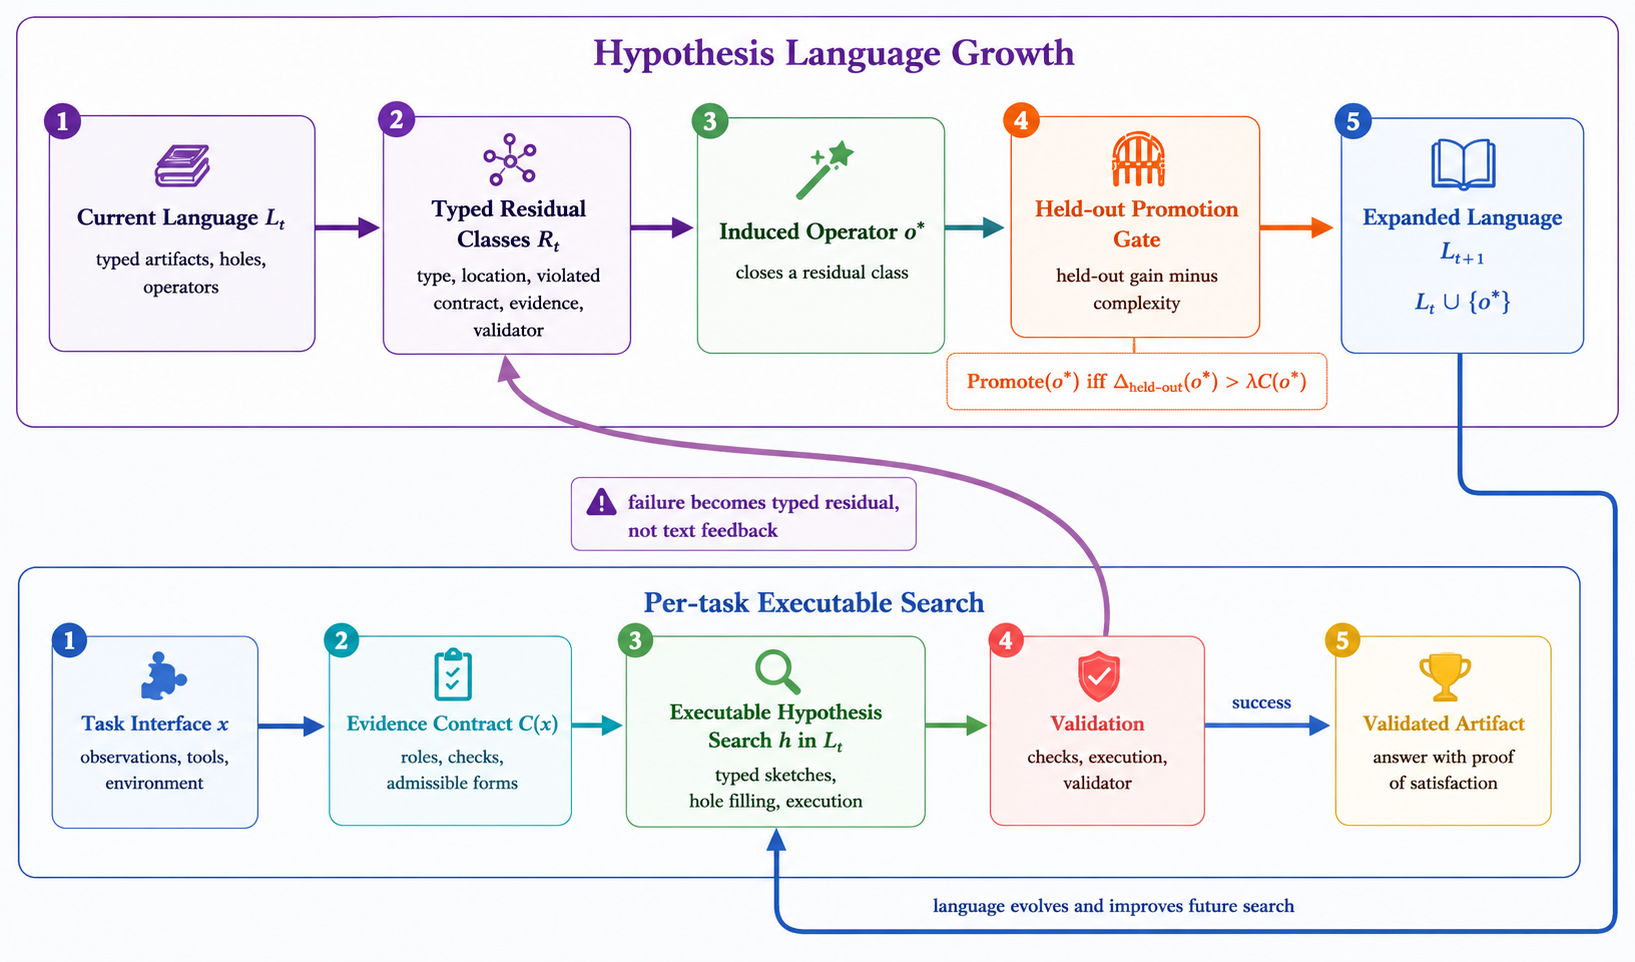
\includegraphics[width=0.98\textwidth]{paper_assets/figures/hypothesis_language_growth_pipeline.png}
\caption{Hypothesis-language growth in \methodshort. The lower loop constructs
and validates an artifact for the current task. A failed validation becomes a
typed residual rather than textual feedback. The upper loop admits a reusable
operator only when it improves held-out utility beyond its complexity cost,
thereby changing the language available to later tasks.}
\label{fig:rghli_architecture}
\end{figure*}

Figure~\ref{fig:rghli_architecture} separates the two time scales of the
method: per-task search produces a validated artifact, while development-time
residual induction may change the language in which later searches operate.

\subsection{The \textsc{HypothesisContext}}

For a task $x$, the context is
\begin{equation}
  \mathcal{M}_x=(C,\mathcal{H},\Theta,\mathcal{E},
  \mathcal{R},\mathcal{O},h^\star),
\end{equation}
where $C$ is the evidence contract, $\mathcal{H}$ is the pool of candidate
artifacts, $\Theta$ stores closed typed holes, $\mathcal{E}$ stores executable
evidence, $\mathcal{R}$ stores typed residuals, $\mathcal{O}$ is the active
operator set, and $h^\star$ is the current best answer artifact. All operators
read and write this object. This is the main architectural constraint: every
stage must return a state update, not a private chain of thought.

Each operator $O_j\in\mathcal{O}$ has the same interface,
\begin{equation}
  O_j(\mathcal{M}_x,x) \rightarrow
  \{(h,e,\rho,\Delta\mathcal{M})\},
\end{equation}
where $h$ is a proposed artifact, $e$ is executed evidence, $\rho$ is the typed
residual, and $\Delta\mathcal{M}$ is the state update. This interface is what
makes the system benchmark-independent. A tabular estimand, a symbolic
coordinate probe, and a transition-rule inducer differ internally, but the
kernel only sees artifact, evidence, residual, and update.

\paragraph{Candidate scoring and typed residuals.}
The kernel ranks candidates by a shared energy score:
\begin{equation}
\begin{aligned}
  \operatorname{score}(h)
  ={}& \lambda_E E(h,x)
  + \lambda_C \operatorname{cover}(h,C) \\
  &- \lambda_V V(h,C)
  - \lambda_H K_h(h).
\end{aligned}
\end{equation}
This objective is Bayesian in motivation--evidence should increase confidence,
while instability and complexity should decrease it--but we do not require a
calibrated likelihood or learned prior. The operational object is the
benchmark-independent energy decomposition and the typed residual emitted when
that score fails. The same decomposition is used across interfaces,
while each operator normalizes its executable evidence to a comparable range
before entering the shared ranking function. The fixed term definitions,
ranges, and weights are reported in the supplement.

\paragraph{End-to-end trace.}
In a NewtonBench-style trajectory, the model does not guess the law directly:
the contract asks for coordinate, exponent, constant, and residual slots; a
sketch $y=c\phi(x)^p$ is executed; residual curvature activates a coordinate
probe; the probe closes the coordinate, exponent, and constant slots; and the
held-out validator accepts the artifact. The
failed first probe changes typed state rather than merely changing the next
prompt.

\subsection{Operators}

\paragraph{Contract compiler.}
The contract compiler maps the input interface to required slots and local
validators. It does not predict the gold answer. It predicts what any valid
answer must make observable: answer type, scope, variables, measurement target,
relation form, and rendering constraints.

\paragraph{Typed-hole closure.}
Instead of asking the model for a complete hypothesis, \methodshort asks for sketches
with typed holes and then closes the holes by small executable probes whenever
possible. For a tabular question, a hole may be an outcome role or a window
operator. For a law-discovery task, it may be a coordinate chart or exponent.
For a sequence task, it may be a state variable or transition clause. Closing a
hole adds an assignment to $\Theta$ and reduces the search space for later
holes.

\paragraph{Executable estimands and coordinate probes.}
The estimand operator creates statistical objects for tabular discovery:
group contrasts, interaction effects, coefficient shifts, multi-item
proportions, and time-window measurements. The coordinate-probe operator
creates compact transformations for laws and rules: log-log fits, affine and
polynomial lifts, ratios, finite differences, thresholds, and simple
state-transition clauses. Both operators produce evidence objects rather than
only prose rationales.

\paragraph{Metamorphic verifier.}
The verifier checks whether the artifact answers the requested question under
transformations that should preserve the object: renaming irrelevant columns,
holding answer form fixed, changing display order, perturbing nuisance values,
or replaying held-out traces. These checks are label-free and therefore
available before benchmark evaluation.

\subsection{Induction Algorithms}

The procedure runs at two time scales. At benchmark time, the language
$L^\star$ is frozen. The system compiles $C_x$, initializes
$\mathcal{M}_x$, repeatedly selects admissible operators, executes their
probes, writes artifacts/evidence/residuals back into the context, updates
$h^\star$ by the shared score, and finally renders $R_x(h^\star)$. Residuals
from reported test rows may be logged for analysis, but they cannot change
$L^\star$ for later reported rows. At development time, residuals are
canonicalized and grouped by residual type, location class, contract role, and
evidence geometry. The reported mechanism audit uses deterministic signatures
and requires at least two compatible source residuals. Each recurrent class may
propose a candidate operator through the same small-model code-and-sketch
interface used for task solving. The operator is discarded unless it passes
static type checks, sandbox execution, validators, and the held-out promotion
rule below. Full pseudocode is provided in the supplement.

\paragraph{Language-growth protocol.}
The promotion step has two modes. During development, residuals may induce
candidate operators, which are promoted only if they improve a held-out
development set after the complexity penalty in Eq.~\eqref{eq:promotion}. For the headline
benchmark runs, the resulting operator language $L^\star$ is frozen before the
reported evaluation. The benchmark score is never used as the promotion signal
for examples later reported as test results. Online adaptation is therefore
limited to per-task hypothesis search in the frozen language, not to changing
the language using future test labels.

\begin{figure*}[t]
\centering
\setlength{\fboxsep}{6pt}
\fcolorbox{gridline}{controlrow}{%
\begin{minipage}{0.95\textwidth}
\small
\textbf{A retained NewtonBench language-growth trace}\\[-1pt]
\rule{\linewidth}{0.3pt}\\[-2pt]
\begin{tabularx}{\linewidth}{@{}p{0.18\linewidth}Y@{}}
\textsc{Development evidence} & Gravity and Coulomb modules both leave the
same typed residual: a positive structured relation cannot be closed in the
current coordinate system. \\
\textsc{Residual-conditioned proposal} & Propose a log-coordinate operator
that fits exponents by execution: $\log y=a+\sum_i p_i\log x_i$. The operator
is a typed transform with declared inputs, output form, and validators. \\
\textsc{Held-out promotion} & Evaluate the transform on disjoint promotion
modules and subtract its program-complexity cost. The utility is positive, so
the operator is added to $L_{t+1}$ rather than stored as a solved example. \\
\textsc{Disjoint transfer} & On the unseen Hooke module, the extended language
exposes the force--displacement family and lowers executable loss from
$1.000$ to $0.206$, with no new operator induction. \\
\end{tabularx}
\end{minipage}}
\caption{An audited, concrete language-growth step. The persistent object is a
small executable coordinate transform, not a Gravity, Coulomb, or Hooke answer
cached for reuse.}
\label{fig:newton_text_exhibit}
\end{figure*}

\paragraph{Running example.}
Figure~\ref{fig:newton_text_exhibit} traces the first accepted NewtonBench
extension in the frozen audit. It illustrates the intended separation: repeated
failures identify an operator class; held-out utility decides promotion; and a
disjoint task benefits from the changed hypothesis language.

\subsection{Residual-Conditioned Operator Promotion}

The residual-extension step is not arbitrary code growth. A residual cluster
$R=\{\rho_1,\ldots,\rho_m\}$ can propose an operator only if it identifies a
repeatable missing transformation. Formally, a candidate operator $O'$ is
promoted when
\begin{equation}
\begin{aligned}
  G(O') ={}&
  \mathbb{E}_{x\sim\mathcal{D}_{held}}
  [U_x(h^\star_{O'}(x))-U_x(h^\star(x))] \\
  &-\beta K_o(O') > 0,
\end{aligned}
\label{eq:promotion}
\end{equation}
where $U_x$ is a development-time executable validation utility, not the
reported benchmark evaluator $S_x$. Source and promotion tasks are disjoint,
and at least one promotion interface must improve. All promotable transforms
are serialized into a common executable intermediate representation, with
$K_o(O')=\log(1+n_{\mathrm{AST}}(O'))$. We fix $\beta=10^{-3}$ before the
reported trajectory. This rule limits uncontrolled library growth: an operator
must improve non-source tasks under the same validation interface while paying
a complexity penalty.

\subsection{Why This Helps Small Models}

\methodshort changes the role of the language model. The model does not need to hold
the entire long-horizon proof in context or invent the final hypothesis in one
sample. It repeatedly proposes local typed objects whose consequences can be
executed. Each closed hole constrains later holes, each verifier rejects an
invalid answer form before final scoring, and each residual becomes a structured
training signal for the outer loop. The intended gain is therefore not more
 verbal reasoning, but a better external search geometry for capacity-limited models.

\section{Experimental Evaluation}

\subsection{Benchmarks and protocol}

We evaluate on three benchmark families that stress different scientific
interfaces while sharing the same central difficulty: the agent must construct
a hypothesis object before it can answer. DiscoveryBench provides real
datasets, metadata, and natural-language discovery goals; the final answer is
scored by Hypothesis Matching Score (HMS) and a consistency-HMS variant.
NewtonBench provides interactive scientific-law discovery tasks in shifted
physical worlds; we report symbolic accuracy over all tasks (SA-all) and over
non-abstained answers (SA-answered). UltraHorizon provides long-horizon
partially observable rule-induction environments; we report the reproduced
paper-style environment score.

The reported system uses a \gptmini core throughout. We use one shared
hypothesis-induction stack: contract compilation, typed-hole closure,
estimand synthesis, coordinate probing, metamorphic validation, and
residual-conditioned promotion. Benchmark adapters expose observations,
validators, and final renderers; interface-specific operator families expose
measurable objects appropriate to each environment, but they all write the same
\textsc{HypothesisContext} and obey the same residual and promotion interface.
Because the artifact types differ, evaluation uses a separately frozen
$L^\star_{\mathrm{DB}}$, $L^\star_{\mathrm{NB}}$, and
$L^\star_{\mathrm{UH}}$, rather than claiming one identical operator library.
We use ``small'' operationally to denote the lower-cost \gptmini proposal tier,
not an undisclosed parameter-count threshold.
We exclude diagnostic ceiling runs that used task-family measurement
bootstraps or hand-engineered rendering fixes.

Complete row counts, evaluator configurations, confidence intervals, and the
frozen-language protocol are reported in the supplement. In particular, the
UltraHorizon result uses the strict configuration, with fallback commits,
environment hints, terminal controllers, and measurement bootstraps disabled.

\subsection{Main comparisons}

Table~\ref{tab:main_results} reports the complete benchmark runs together with
published original-paper references and local controls. Published rows are
contextual reference points. Where a matched local baseline is available, it
uses the same proposal core, task set, and evaluator as \methodshort within its
benchmark block; the strict UltraHorizon control instead isolates the shared
kernel from its optional components. All \methodshort operator languages are
frozen before reported evaluation. The canonical NewtonBench result therefore
evaluates the typed executable kernel, while development-time language growth is
tested separately below.

\begin{table*}[t]
\centering
\caption{Complete benchmark comparisons. Scores use each benchmark's native
metric and are comparable only within a benchmark block. ``Paper'' rows are
results reported in the original benchmark papers; local rows are our complete
evaluations. The DiscoveryBench Reflexion row uses oracle feedback and is shown
only as contextual reference. Intervals are 95\% nonparametric bootstrap intervals.}
\label{tab:main_results}
\footnotesize
\renewcommand{\arraystretch}{1.12}
\setlength{\tabcolsep}{4pt}
\begin{tabularx}{0.82\textwidth}{|Y|c|c|}
\hline
\tblhdr
Method & Core & Native score \\
\hline
\rowcolor{headerrow}
\multicolumn{3}{|l|}{\textit{DiscoveryBench: HMS \citep{discoverybench}}} \\
\hline
\rowcolor{cautionrow}
CodeGen (paper) & GPT-4-preview & 16.3 \\
\hline
\rowcolor{cautionrow}
\react (paper) & GPT-4-preview & 15.6 \\
\hline
\rowcolor{cautionrow}
Reflexion (oracle; paper) & GPT-4o & 24.5 \\
\hline
\rowcolor{controlrow}
Direct & \gptmini & 9.54 \\
\hline
\rowcolor{controlrow}
\react & \gptmini & 11.68 \\
\hline
\rowcolor{controlrow}
\codeact & \gptmini & 12.31 \\
\hline
\rowcolor{rghlirow}
\methodshort & \gptmini & \textbf{28.70} [23.24, 34.28] \\
\hline
\rowcolor{headerrow}
\multicolumn{3}{|l|}{\textit{NewtonBench: SA-all (\%) \citep{newtonbench}}} \\
\hline
\rowcolor{cautionrow}
Best paper result & GPT-5 & 75.9 \\
\hline
\rowcolor{cautionrow}
Small-model paper reference & o4-mini & 47.8 \\
\hline
\rowcolor{controlrow}
Vanilla/ReAct-like & \gptmini & 0.00 \\
\hline
\rowcolor{controlrow}
\codeact & \gptmini & 0.62 \\
\hline
\rowcolor{rghlirow}
\methodshort & \gptmini & \textbf{49.38} [44.14, 54.94] \\
\hline
\rowcolor{headerrow}
\multicolumn{3}{|l|}{\textit{UltraHorizon: environment score \citep{ultrahorizon}}} \\
\hline
\rowcolor{cautionrow}
Best paper LLM, free steps & Gemini-2.5-Pro & 14.33 \\
\hline
\rowcolor{cautionrow}
Human participants (paper) & human & 26.52 \\
\hline
\rowcolor{controlrow}
All-off strict (ours) & \gptmini & 0.00 \\
\hline
\rowcolor{rghlirow}
\methodshort strict & \gptmini & \textbf{51.04} [44.79, 56.88] \\
\hline
\end{tabularx}
\end{table*}

\begin{figure*}[t]
\centering
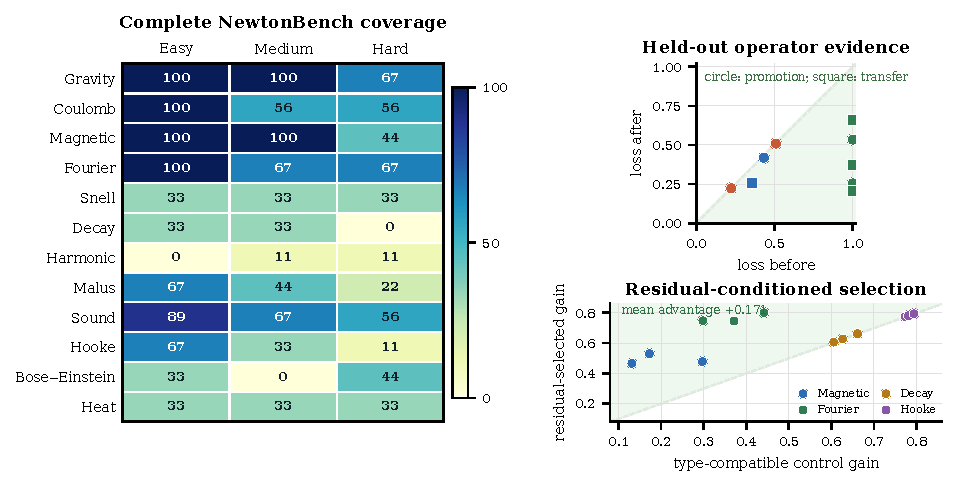
\includegraphics[width=0.94\textwidth]{paper_assets/figures/newton_coverage_growth_composite.pdf}
\caption{Complete NewtonBench coverage and the frozen language-growth audit.
Left: exact symbolic accuracy over all 324 task configurations; each cell
averages three law versions and three system variants. Upper right: executable
loss before and after accepted operators on held-out promotion and disjoint
transfer interfaces. Lower right: 12 paired evaluations compare the
residual-selected family with a type-compatible control under identical
fitting and test-time compute; points above the diagonal favor residual
conditioning.}
\label{fig:newton_coverage_growth}
\end{figure*}

\clearpage

\subsection{Mechanism evidence}

\enlargethispage{\dimexpr\textheight-\pagegoal\relax}
The benchmark table establishes a system-level comparison, but not the source
of the gain. We therefore freeze observations, parameter fitting, and
test-time model calls in a NewtonBench diagnostic. Residual-conditioned
selection reduces held-out executable loss by $0.171\pm0.012$ relative to a
type-compatible additive control. This estimate contains 12 paired task
evaluations: four held-out physical-law interfaces under three independently
seeded splits. Figure~\ref{fig:newton_coverage_growth} shows both the complete
324-task profile and the disjoint evidence behind the admitted extensions.
The matched controls produce parseable candidate laws and pass the same parser
and judge; the supplement gives prompts, category audit, and representative
traces.

\subsection{What the full runs show}

The full runs test one typed-state kernel across three scientific interfaces.
DiscoveryBench reaches 28.70 HMS, versus 9.54--12.31 for matched Direct,
\react, and \codeact controls. NewtonBench reaches 49.38\% SA-all at 74.1\%
coverage; matched interactive and code-action controls reach 0.00\% and 0.62\%.
On UltraHorizon, the strict configuration preserves an induced program across a
fixed 50-step horizon and reaches 51.04. The state schema and promotion
interface are shared, while each benchmark freezes a language appropriate to
its artifact type. Separate frozen-transfer and multi-step audits test language
growth; the supplement provides residual taxonomies, provenance, and traces.

These experiments separate system-level utility from the mechanism claim. The
complete runs use native evaluators, paired controls fix the task set, backbone,
parser, and evaluator, and the disjoint audit tests transfer across interfaces.
Because admission requires held-out loss reduction after a complexity charge,
the $0.171\pm0.012$ advantage and the accepted--rejected updates in
Figure~\ref{fig:newton_coverage_growth} and the audited trace below specifically
test language growth.

\par\medskip
\noindent
\setlength{\fboxsep}{5pt}
\fcolorbox{gridline}{controlrow}{%
\begin{minipage}{0.91\columnwidth}
\footnotesize
\textbf{One audited language update.}
Gravity and Coulomb interfaces produced a recurrent positive, log-structured
residual class. The residual-conditioned proposal was a positive-monomial
lattice:
\[
L_0 \xrightarrow[\;0.6055-0.0067=+0.5988\;]{\text{held-out promotion}}
L_1=L_0\cup\{o_{\mathrm{mono}}\}.
\]
After freezing $L_1$, the operator reduced executable loss by $0.5871$ on
disjoint transfer interfaces. A repeated copy later had net gain $-0.0067$ and
was rejected. Admission used disjoint executable loss plus the declared
complexity charge; benchmark scores and reported-test residuals were
unavailable to the gate.
\medskip

{\scriptsize
\begin{tabularx}{\linewidth}{@{}lXr@{}}
\toprule
Update & Disjoint evidence & Outcome \\
\midrule
$L_0\!\to\!L_1$ & gravity, Coulomb $\to$ magnetic, Fourier
  & $+0.5988$ \\
frozen $L_1$ & decay, Hooke, heat-transfer
  & $+0.5871$ \\
$L_1\!\to\!L_2$ & underdamped, Malus $\to$ sound-speed
  & $+0.0082$ \\
frozen $L_2$ & Bose--Einstein distribution
  & $+0.0996$ \\
duplicate & repeated monomial source hash
  & $-0.0067$ \\
\bottomrule
\end{tabularx}}
\smallskip
\noindent\scriptsize\textit{The admitted operator changes the executable
search space before transfer; recurrence alone does not guarantee promotion,
and the language is frozen before reported rows.}
\end{minipage}}
\par\smallskip

\section{Limitations}

\methodshort assumes that scientific intermediates admit executable contracts,
typed holes, validators, renderers, or residual-induced operators. The current
implementation covers three artifact classes and uses fixed energy weights;
richer semantic renderers and learned held-out calibration remain open.

The benchmarks intentionally use different evaluators. DiscoveryBench rewards
semantic agreement, NewtonBench rewards symbolic equivalence, and UltraHorizon
rewards long-horizon behavior. We therefore report native metrics rather than
collapsing them into one aggregate. The common object is the frozen typed-state
and operator protocol, not one identical operator library. The UltraHorizon
strict result demonstrates the interface on Grid and Seq but does not solve Bio
or provide an external-agent matched control.

RG-HLI deliberately promotes only small operators that can be serialized,
executed, and tested on disjoint interfaces. It is therefore a method for
making representational growth inspectable rather than a claim that every
scientific concept can be reduced to a short program. In settings where the
critical abstraction has no executable evidence or validator, the system
retains an auditable unresolved residual instead of treating a plausible verbal
repair as a new capability. This constraint is useful in practice: it makes the
next target explicit and prevents a solved-looking trajectory from silently
becoming library state.

Reported-test residuals, benchmark scores, and gold laws are unavailable to the
promotion gate and cannot rewrite the frozen language.

Matched comparisons hold the proposal backbone, task set, parser, and evaluator
fixed, but structured execution uses more calls than direct prompting. The
supplement reports retained call records where available and complete run
provenance; our claim is architectural utility at the stated budget, not a
compute-matched Pareto frontier. Since the provider does not disclose parameter
count, ``small'' denotes the compact, low-cost proposal tier rather than a
parameter threshold.

NewtonBench SA-all is the primary metric and counts abstentions as errors; the
system answers 74.1\% of tasks. We report SA-answered and coverage separately in
the supplement so that precision cannot be improved invisibly by abstention.
For UltraHorizon, the headline strict run excludes the public terminal
controller and reports the internal executor without a controller-assisted
score.

\section{Conclusion}

\methodshort turns validation failures into typed, executable language growth:
held-out promotion creates auditable operators whose frozen transfer
distinguishes expanded hypothesis spaces from additional search. Complete
native-evaluator runs show one typed-state kernel operating across tabular
discovery, symbolic laws, and long-horizon rules, while the accepted--rejected
trajectory isolates representational growth from extra inference steps.
\newpage
\bibliography{residual_guided_hli_refs}

\end{document}
